\section{Controlador Local - Morpheus \label{chap:morpheus}}

\subsection{Descrição}
Morpheus é o servidor local responsável pela interconexão da casa inteligente com os serviços de nuvem. O nome tem sua origem na mitologia grega, cujo Deus dos sonhos, Morpheus, era responsável pelo envio de mensagens entre dois mundos diferentes, o dos deuses e o dos mortais \cite{morpheusName}. A principal atribuição do servidor local é garantir que a troca de mensagem entre os módulos e a nuvem seja realizada com segurança e confiabilidade, munindo-se de soluções robustas para desempenhar o seu papel.

\subsection{Plataforma}
O Morpheus tem seu desenvolvimento realizado em Java. Conforme será detalhado em seguida, tal escolha foi realizada com base na portabilidade que a máquina virtual Java (JVM) oferece, bem como na disponibilidade de bibliotecas e serviços largamente utilizados em aplicações comerciais. O servidor foi construído utilizando-se o Spring Boot Framework.

Para se comunicar com os módulos, o Morpheus utiliza-se da conexão com um \emph{broker} \wmqtt{}. O \emph{broker} Mosquitto foi utilizado por ser uma solução \emph{open-source} largamente utilizada em projetos de \wiot. Conforme detalhado a frente, configurações de segurança específicas para o projeto foram registradas no \emph{broker}. Para a conexão com os serviços na nuvem, é utilizado um canal WebSocket aberto pelo Morpheus (cliente) e aceito pela nuvem (servidor). Esta solução veio a partir de uma discussão em relação à segurança, relativa ao requisito não-funcional RNF-6, conforme documentada na Subseção \ref{sub:websocket}.

\subsection{Tecnologias Utilizadas}
Toda a implementação do Morpheus foi realizada na linguagem Java. Desde o começo do projeto, decidiu-se que a escolha de tecnologias para implementação das diversas camadas deveria ter por base os seus benefícios, e não necessitaria ser rígida ou uniforme. Assim, o principal esforço foi sempre no planejamento das interfaces de comunicação entre as partes, que poderiam ser implementadas em linguagens complementamente diferentes. Os sistemas de nuvem, por exemplo, foram implementados em Node.js. O aplicativo web também em foi feito em JavaScript, com utilização da biblioteca React. Os módulos de hardware foram programados em linguagem \emph{C-like}, própria para Arduino, e o controlador local em Java. Essa flexibilidade permitiu a utilização de recursos e tecnologias que fossem melhor integrados com os requisitos propostos.

Um requisito essencial para o controlador local é a sua robustez (RNF-4). Em um cenário em que este controlador não esteja disponível, a casa passa a funcionar em estado de emergência, no qual os comandos são reduzidos e não permitem acesso remoto. Entretanto, há inúmeras possibilidades e eventos que poderiam causar a queda deste controlador, muitas das quais referem-se a situações fora de nosso alcance. Por exemplo, a falta de energia ou de Internet na residência interrompe o seu funcionamento, não sendo possível ter controle sobre tal situação. O mesmo ocorre no evento de problemas de hardware na plataforma que o sistema estiver rodando. Os planos para contenção dos seus efeitos de tais situações são complexos, custosos e fogem do escopo deste projeto, como seria o caso de implementar duplicações, banco de baterias e tecnologia celular para comunicação secundária.

Há, entretanto, problemas no software que poderiam afetar o funcionamento do controlador. Por meio de testes, muitos desses problemas podem ser evitados ainda em tempo de desenvolvimento. A utilização de tecnologias que facilitam o desenvolvimento seguro da aplicação é uma vantagem para este caso, já que ferramentas estão disponíveis para que haja maior controle sobre o código desenvolvido, e pode-se detectar erros mais facilmente, ainda em tempo de compilação, por exemplo.

O controlador local também precisa lidar com as requisições assincronamente, conforme o requisito não-funcional RNF-10. Parte desta tarefa é facilitada com a utilização do sistema de mensageria \wmqtt{}, operado pelo \emph{broker} Mosquitto. Com sua utilização, mensagens podem ser enviadas mesmo que o controlador não consiga recebê-las, pois elas não serão perdidas. Entretanto, devido às características do sistema proposto, as mensagens precisam ser operadas sem maiores demoras. O controlador deve receber e processar as mensagens paralelamente, e não esperar o processamento de uma mensagem inteira para processar a próxima, de modo que o paralelismo deve ser parte essencial da arquitetura.

Ainda, para a integração com os serviços da nuvem, é necessário a utilização de JSON, para a serialização das mensagens, em um formato que pode ser desserializado posteriormente, independentemente da plataforma. Para a utilização de WebSockets, é necessário o uso de bibliotecas disponíveis, de modo que o desenvolvimento seja facilitado. Por último, é necessário gerenciar eficientemente todas essas dependências. Atualizá-las quando necessário, ou substituí-las, se desejado, deve ser uma tarefa simples.

A arquitetura oferecida pelo Java mostra ser efetiva para as necessidades levantadas acima. Com a utilização de uma IDE avançada, inúmeros recursos estão disponíveis para limpeza, refatoração, organização do código, etc. É uma linguagem utilizada em vasta gama de aplicações, desde complexos softwares comerciais como a IDE Eclipse, até softwares embutidos, como controladores de BlueRay \cite{javaBlueray}. A escolha do Java 8 foi decidida para que o desenvolvimento possa utilizar certos recursos de paradigmas funcionais, como o conceito de Streams de dados e Funções Lambdas.

O \emph{framework} Spring Boot\footnote{https://projects.spring.io/spring-boot/} foi utilizado para o desenvolvimento por oferecer diversos recursos facilitadores, configurações de ambiente e um \emph{container} para inversão de controle (\emph{IoC - Inversion of Control}) e injeção de dependência. Essa técnica diminui o acoplamento entre classes e permite a evolução e implementação de novas funcionalidades de maneira fácil \cite{iocFowler}. Assim, cada módulo recebe em seu construtor todas as dependências que serão utilizadas. A responsabilidade da construção de tais dependências passa, então, a ser responsabilidade do gerenciador de contexto, e não mais do módulo.

Além disso, o gerenciador de dependências Gradle\footnote{https://gradle.org/} também foi utilizado por oferecer um poderoso ambiente para configurar, construir e distribuir aplicações. Gradle faz uso de Groovy\footnote{http://groovy-lang.org/}, tecnologia que também roda na Java Virtual Machine (JVM). Por outro lado, o uso de tais ferramentas e plataformas necessita de hardware mais robusto para que funcione, sendo uma desvantagem. Contudo, frente aos benefícios, ainda é vantajosa a utilização de Java neste caso.

Internamente, o Morpheus é dividido em pacotes, que são responsáveis pela modelagem do problema. Há classes que modelam o domínio, que executam as regras de negócio, que fazem a interface entre outros sistemas (\wmqtt{} Mosquitto Broker e nuvem), e que fazem a execução de tarefas como backup de mensagens, e serviços de conversão.
Assim que uma mensagem chega ao Morpheus, ela é reconhecida e é realizado o seu \emph{parsing} para as estruturas de domínio internas. Caso haja algum erro nas mensagens vindas da nuvem, há o envio de relatório com os problemas encontrados. A partir do reconhecimento, a mensagem é colocada em uma fila interna, onde outro módulo será responsável por capturá-la e realizar o processamento necessário.

\begin{figure}
	\centering
	\caption{Arquitetura do servidor local}
  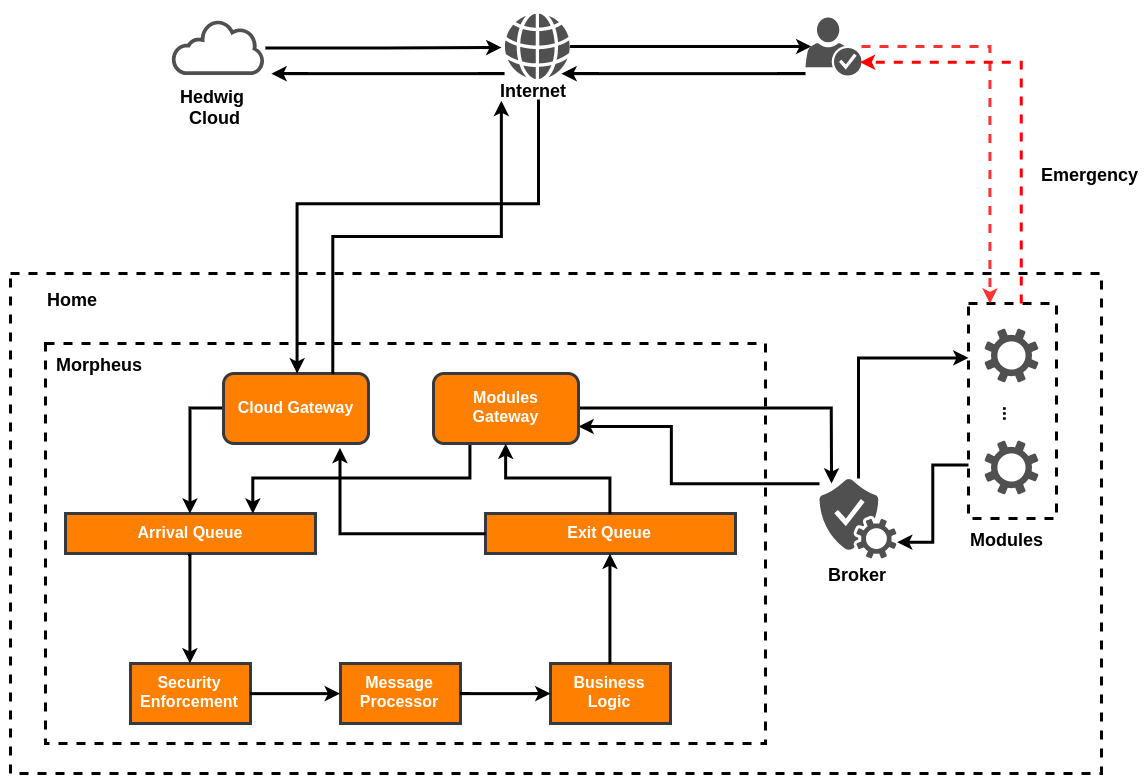
\includegraphics[width=\textwidth]{diagramaDeComunicacao}
\label{fig:diagramaDeComunicacao}
\end{figure}

\subsection{Características e Recursos}
Para a concepção do servidor local, foram considerados os requisitos funcionais e não-funcionais, discutidos na Seção \ref{sec:requisitos}. As características e recursos da implementação são discutidos em seguida.

\begin{description}

\item \textbf{Configuração dos módulos físicos}

De acordo com as regras e interfaces estabelecidas, os módulos podem ser configurados por meio de mensagens. Os serviços da nuvem enviam os parâmetros de configuração de cada módulo ao Morpheus, que os transmitirá ao módulo.

\item \textbf{Envio de dados para a nuvem}

Dados provenientes de sensores são enviados para a nuvem, para que possam ser tratados de acordo com as regras de \emph{Business Intelligence} e utilizados em algoritmos de aprendizado de máquina.

\item \textbf{Persistência de dados}

Quando não houver conexão, o servidor armazena os dados localmente e, quando solicitado, os envia à nuvem.

\item \textbf{Tentativas de reenvio}

Quando uma mensagem não é enviada com sucesso à nuvem, o Morpheus tenta novamente por um número configurável de vezes em um curto espaço de tempo. Isso ocorre porque, se determinada mensagem não pode ser enviada em uma janela temporal, ela perde o seu sentido (e.g. requisição de abertura de portão).

\item \textbf{Verificação do \emph{timestamp}}

Quando uma nova mensagem chegar, seu \emph{timestamp} é verificado, e a mensagem tomará curso somente se não for obsoleta.

\item \textbf{Tomadas de ação}

Quando o usuário requisitar uma tomada de ação, esta deve ser enviada por meio de uma mensagem ao Morpheus, por onde será transmitida ao módulo.

\item \textbf{Configuração em arquivo}

As configurações básicas do Morpheus devem ser registradas em um arquivo YAML que é lido durante a inicialização.

\item \textbf{Listeners para diferentes tipos de mensagens}

Devem haver \emph{listeners} para todos os tipos de mensagens que são recebidos da nuvem e dos módulos.

\item \textbf{Processamento concorrente}

Toda a infraestrutura do Morpheus permite o processamento concorrente de mensagens. Não é necessário esperar o processamento completo de uma mensagem para que outra comece a ser processada.

\item \textbf{Utilização de criptografia na troca de mensagens com a nuvem}

Os dados que trafegam entre a nuvem e o servidor local são encriptados na camada de transporte por meio de \emph{TLS}.

\item \textbf{Conversão de mensagens}

As mensagens enviadas à nuvem são codificadas em JSON após serem convertidas do formato interno, que se refere apenas à troca de mensagens entre os módulos e o Morpheus.

\item \textbf{Serialização das configurações}

O servidor serializa e persiste as configurações relativas aos módulos que foram configurados para carregá-las em sua inicialização.

\item \textbf{Destruição de pools de threads}

Ao ser desligado, todos os \emph{pools} de \emph{threads} criados são destruídos.

\end{description}

\subsection{Protocolo para Troca de Mensagens com Módulos}

Toda a comunicação entre as partes do projeto é realizada por troca de mensagens. Foi desenvolvido um protocolo específico, leve e expansível, para a codificação dessas mensagens. As subseções seguintes definem e exemplificam o uso do protocolo.

\subsubsection{Tópicos}
Todos os tópicos devem seguir o formato especificado em seguida. Com essa formatação, é possível garantir que:

\begin{enumerate}
\item Somente o Morpheus consegue publicar em qualquer tópico ou ser um \emph{subscriber} de qualquer tópico.
\item Cada módulo somente consigue publicar no tópico determinado para ele, o que é garantido com as credenciais (usuário e senha) fornecidos pelo tópico.
\item Caso um módulo malicioso seja implantado com o roubo das credenciais de um módulo legítimo, o impacto será unicamente concentrado naquele tópico, não atingindo outros módulos.
\end{enumerate}

Têm-se as seguintes regras:

\textbf{hw/\textless ID do módulo\textgreater /s2m}

\emph{Server to Module} --- o módulo deve ser \emph{subscriber} desse tópico. O servidor deve ser \emph{publisher} desse tópico.

\textbf{hw/\textless ID do módulo\textgreater /m2s}

\emph{Module to Server} --- o servidor deve ser \emph{subscriber} desse tópico. O módulo deve ser \emph{publisher} desse tópico.

\subsubsection{Regras de Negócio}
O servidor foi desenvolvido com base nas regras de negócio seguintes. Cada regra de negócio tem sua identificação dada por \emph{mRN}, seguida de um identificador numérico --- e.g. \emph{mRN-1}.
\begin{description}
\item[mRN-1:]Após a compra de cada módulo, o usuário deve registrar online a aquisição. O servidor da nuvem enviará para o servidor local da casa a requisição para configurar o módulo.
\item[mRN-2:]Cada módulo envia mensagens para o servidor local com o seus dados por meio do \wmqtt{}.
\item[mRN-3:]Para a troca de senha do Wi-Fi, o usuário cadastra no aplicativo a nova senha. O servidor na nuvem faz a requisição para o servidor local, o qual enviará um arquivo de configuração com a nova senha para cada um dos módulos registrados. Após a configuração de todos os módulos, o servidor local envia resposta de sucesso para a nuvem, a qual indica ao usuário que a troca de senha já pode ser feita com sucesso.
\item[mRN-4:]Todo módulo sai de fábrica configurado com o tópico que deve se inscrever e publicar com base no seu ID, o qual será o seu usuário, também havendo uma senha para se autenticar junto ao \emph{broker} \wmqtt{}.
\end{description}

\subsubsection{Definição de Interfaces}
\begin{itemize}
\item Há três tipos de mensagens que vão do Morpheus para os módulos:
  \begin{itemize}
  \item Configuração (\texttt{configuration})
  \item Requisição de ação (\texttt{action\_request})
  \item Requisição de dados (\texttt{data\_transmission})
  \end{itemize}
\item Há três tipos de mensagens que chegam dos módulos:
  \begin{itemize}
  \item Confirmação (\texttt{confirmation})
  \item Envio de dados (\texttt{data\_transmission})
  \item Requisição de dados (\texttt{data\_request})
  \end{itemize}
\end{itemize}

\subsubsection{Definição das Mensagens}

\paragraph{Configuração (\texttt{configuration})}
\begin{itemize}
\item Sentido: Morpheus para módulo.
\item Uso: envio de parâmetros para configuração dos módulos.
\end{itemize}

\textbf{Configuração de hora}
\begin{lstlisting}
#configuration
$ts: <timestamp>
$ty: time_config
@
updated_ntp: <segundos desde 00h00 de 1 de Janeiro de 1970, 64 bits>
@
\end{lstlisting}

\textbf{Configuração de nome}
\begin{lstlisting}
#configuration
$ts: <timestamp>
$ty: name_config
@
new_name: <string do nome>
new_rele1name: <string do nome | "">
new_rele2name: <string do nome | "">
@
\end{lstlisting}

\textbf{Configuração de comunicação}
\begin{lstlisting}
#configuration
$ts: <timestamp>
$ty: comunication_config
@
new_ssid: <novo ssid>
new_password: <nova senha>
ip_local: <novo ip local fixo>
ap_mod: <"sempre ativo" | "automatico">
ap_name: <nome do ap para acesso direto>
ap_password: <senha do ap para acesso direto>
@
\end{lstlisting}

\textbf{Configuração de RF}
\begin{lstlisting}
#configuration
$ts: <timestamp>
$ty: rf_config
@
<nome do sensor | controle | funcao>: <"store" | "clear" | "keep">
@
\end{lstlisting}

\textbf{Configuração de display}
\begin{lstlisting}
#configuration
$ts: <timestamp>
$ty: display_config
@
displaytype: <1 | 2 | 3>
backlight: <0 | 1 | 2>
@
\end{lstlisting}
0 = desligado, 1 = ligado, 2 = automático

\paragraph{Requisição de ação (\texttt{action\_request})}
\begin{itemize}
\item Sentido: Morpheus para módulo.
\item Uso: quando um usuário faz a requisição de uma ação por meio do aplicativo. Por exemplo, quando deseja-se acender uma luz, o aplicativo envia uma requisição para o Morpheus, que enviará uma mensagem de \texttt{action\_request} para o módulo correspondente.
\end{itemize}

\textbf{Requisição de acionamento}
\begin{lstlisting}
#action_request
$ts: <timestamp>
$ty: rele1_action
@
rele1: <0 | 1>
@
\end{lstlisting}
Essa mensagem fica sem efeito no caso do Módulo de Acesso, que usa mensagens com senha para o acionamento do relé 1.

Rele1: 0 = desligar; 1 = ligar

\begin{lstlisting}
#action_request
$ts: <timestamp>
$ty: rele2_action
@
rele2: <0 | 1>
@
\end{lstlisting}
Rele2: 0 = desligar; 1 = ligar

\textbf{Requisição de reinício de software}
\begin{lstlisting}
#action_request
$ts: <timestamp>
$ty: sw_reset
@
swreset: <0 | 1>
@
\end{lstlisting}
0 = não; 1 = confirmar reinício

\textbf{Requisição de teste de \emph{auto reset}}
\begin{lstlisting}
#action_request
$ts: <timestamp>
$ty: autoreset_test
@
autoreset: <0 | 1>
@
\end{lstlisting}
0 = não; 1 = confirmar reinício

\paragraph{Confirmação (\texttt{confirmation})}
\begin{itemize}
\item Sentido: do módulo para o servidor.
\item Uso: confirmação de uma configuração ou requisição de ação vindas do servidor.
\end{itemize}

\textbf{Confirmação de hora}
\begin{lstlisting}
#confirmation
$ts: <timestamp>
$ty: time_confirm
@
ntp: <segundos desde 00h00 de 1 de Janeiro de 1970, 64 bits>
@
\end{lstlisting}

\textbf{Confirmação de nome}
\begin{lstlisting}
#confirmation
$ts: <timestamp>
$ty: name_confirm
@
name: <nome>
rele1name: <string do nome | "">
rele2name: <string do nome | "">
@
\end{lstlisting}

\textbf{Confirmação de comunicação}
\begin{lstlisting}
#confirmation
$ts: <timestamp>
$ty: communication_confirm
@
ssid: <novo ssid>
password: <nova senha>
ip local: <novo ip local fixo>
ap mod: <"sempre ativo" | "automatico">
ap name: <nome do ap para acesso direto>
ap password: <senha do ap para acesso direto>
@
\end{lstlisting}

\textbf{Confirmação de configuração de RF}
\begin{lstlisting}
#confirmation
$ts: <timestamp>
$ty: rf_confirm
@
<nome do sensor | nome do controle | nome do funcao>: <valor_gravado>
@
\end{lstlisting}

\textbf{Configuração de configuração de display}
\begin{lstlisting}
#confirmation
$ts: <timestamp>
$ty: display_confirm
@
displaytype: <1 | 2 | 3>
backlight: <0 | 1>
@
\end{lstlisting}

\textbf{Confirmação de reinício de software}
\begin{lstlisting}
#confirmation
$ts: <timestamp>
$ty: sw_reset_confirm
@
swreset: <0 | 1>
@
\end{lstlisting}

\textbf{Confirmação de teste de \emph{auto reset}}
\begin{lstlisting}
#confirmation
$ts: <timestamp>
$ty: autoreset_test_confirm
@
autoreset: <0 | 1>
@
\end{lstlisting}

\paragraph{Transmissão de dados (\texttt{data\_transmission})}
\begin{itemize}
\item Sentido: do módulo para o servidor.
\item Uso: envio de dados de sensores para o servidor.
\end{itemize}

\textbf{Transmissão de umidade, temperatura, presença, relés, sensor de presença e luminosidade}
\begin{lstlisting}
#data_transmission
$ts: <timestamp>
$ty: temp_umi_pres
@
s1: umidade
vl1: <value>
s2: temperatura
vl2: <value>
s3: presenca
vl3: <value>
s4: rl1
vl4: <value>
s5: rl2
vl5: <value>
s6: abertura
vl6: <0|1>
s7: luz
vl7: <int de 0 a 1000>
@
\end{lstlisting}

\paragraph{Requisição de dados (\texttt{data\_request})}
\begin{itemize}
\item Sentido: do módulo para o servidor.
\item Protocolo: \wmqtt{}
\item Uso: requisição de alguma informação do servidor (ex.: atualização de hora).
\end{itemize}


\textbf{Mensagens próprias para o Módulo de Acesso}


\textbf{Configuração de alarme}
\begin{lstlisting}
#configuration
$ts: <timestamp>
$ty: alarm_config
@
alarme: <0|1>
alarme_tempo: <int do tempo em segundos>
@
\end{lstlisting}

\textbf{Configuração de luz automática}
\begin{lstlisting}
#configuration
$ts: <timestamp>
$ty: auto1_config
@
initial_time1: <integer de 0 a 23>
final_time1: <integer de 0 a 23>
time_keepon1: <tempo em minutos>
time_deslmanual1: <tempo em minutos>
@
\end{lstlisting}

\begin{lstlisting}
#configuration
$ts: <timestamp>
$ty: auto2_config
@
initial_time2: <integer de 0 a 23>
final_time2: <integer de 0 a 23>
time_keepon2: <tempo em minutos>
time_deslmanual2: <tempo em minutos>
@
\end{lstlisting}

\textbf{Configuração de senha}
\begin{lstlisting}
#configuration
$ts: <timestamp>
$ty: password_config
@
old_password: <string>
new_password: <string>
@
\end{lstlisting}

\textbf{Abertura de portão}
\begin{lstlisting}
#action_request
$ts: <timestamp>
$ty: abertura_portao
@
password: <string>
@
\end{lstlisting}

\textbf{Confirmação de alarme}
\begin{lstlisting}
#confirmation
$ts: <timestamp>
$ty: alarm_confirm
@
alarme: <0|1>
alarme_tempo: <tempo em minutos>
@
\end{lstlisting}

\textbf{Confirmação de configuracão de luz automática}
\begin{lstlisting}
#confirmation
$ts: <timestamp>
$ty: auto1_confirm
@
initial_time1: <integer de 0 a 23>
final_time1: <integer de 0 a 23>
time_keepon1: <tempo em minutos>
time_deslmanual1: <tempo em minutos>
@
\end{lstlisting}

\begin{lstlisting}
#confirmation
$ts: <timestamp>
$ty: auto2_confirm
@
initial_time2: <integer de 0 a 23>
final_time2: <integer de 0 a 23>
time_keepon2: <tempo em minutos>
time_deslmanual2: <tempo em minutos>
@
\end{lstlisting}

\textbf{Confirmação de senha}
\begin{lstlisting}
#confirmation
$ts: <timestamp>
$ty: password_confirm
@
password: <string>
@
\end{lstlisting}

\textbf{Transmissão de estado de acesso}
\begin{lstlisting}
#data_transmission
$ts: <timestamp>
$ty: acesso_estado
@
s1: abertura
vl: <0 fechado | 1 aberto>
s2: alarme
vl: <0 desligado | 1 ligado>
s3: tempo_alarme
vl: <value>
@
\end{lstlisting}

tempo\_alarme: tempo em minutos em que o sensor de abertura está aberto.

\textbf{Mensagens próprias para o Módulo do Quarto}

\textbf{Configuração de despertador}
\begin{lstlisting}
#configuration
$ts: <timestamp>
$ty: despertador_config
@
despertador: <0 | 1>
despertador_tempo: <tempo em minutos>
@
\end{lstlisting}

\textbf{Configuração de luz automática}
\begin{lstlisting}
#configuration
$ts: <timestamp>
$ty: acesso_config
@
initial_time: <integer de 0 a 23>
final_time: <integer de 0 a 23>
time_keepon: <tempo em minutos>
time_deslmanual: <tempo em minutos>
@
\end{lstlisting}

\textbf{Confirmação de despertador}
\begin{lstlisting}
#confirmation
$ts: <timestamp>
$ty: despertador_config
@
despertador: <0 | 1>
despertador_tempo: <tempo em minutos>
@
\end{lstlisting}

\textbf{Confirmação de luz automática}
\begin{lstlisting}
$ts: <timestamp>
$ty: acesso_config
@
initial_time: <integer de 0 a 23>
final_time: <integer de 0 a 23>
time_keepon: <tempo em minutos>
time_deslmanual: <tempo em minutos>
\end{lstlisting}

\textbf{Mensagens próprias para o Módulo do Externo}

\textbf{Configuração de alerta de 1 (água) e 2 (energia elétrica)}
\begin{lstlisting}
#configuration
$ts: <timestamp>
$ty: offset_config
@
alerta1: <0 | 1>
alerta1_nivel: <vl>
alerta2: <0 | 1>
alerta2_nivel: <vl>
@
\end{lstlisting}

\textbf{Confirmação de configuração de alerta de 1 (água) e 2 (energia elétrica)}
\begin{lstlisting}
#confirmation
$ts: <timestamp>
$ty: offset_config
@
alerta1: <0 | 1>
alerta1_nivel: <vl>
alerta2: <0 | 1>
alerta2_nivel: <vl>
@
\end{lstlisting}

\textbf{Transmissão de estado de Módulo Externo}
\begin{lstlisting}
#data_transmission
$ts: <timestamp>
$ty: externo_estado
@
s1: agua
vl: <integer>
s2: energia_eletrica
vl: <integer>
s1: agua_alerta
vl: <0 | 1>
s2: energia_eletrica_alerta
vl: <0 | 1>
@
\end{lstlisting}

\textbf{Mensagens próprias para o Módulo da Cozinha}

\textbf{Programação para preparo (café ou arroz)}
\begin{lstlisting}
#configuration
$ts: <timestamp>
$ty: offset_config
@
initialtime: <vl>
finaltime: <vl>
cooking_time: <vl>
cook_mode: <"auto" | "manual">
@
\end{lstlisting}

\textbf{Confirmação de programação para preparo (café ou arroz)}
\begin{lstlisting}
#confirmation
$ts: <timestamp>
$ty: offset_config
@
initialtime: <vl>
finaltime: <vl>
cooking_time: <vl>
cook_mode: <"auto" | "manual">
@
\end{lstlisting}

\textbf{Transmissão de estado do Módulo da Cozinha}
\begin{lstlisting}
#data_transmission
$ts: <timestamp>
$ty: cozinha_estado
@
s1: gas
vl: <integer>
s2: cooking
vl: <0 | 1>
@
\end{lstlisting}

\textbf{Requisição de offset para alarme de gás}
\begin{lstlisting}
#data_transmission
$ts: <timestamp>
$ty: gas_offset
@
<vl>
@
\end{lstlisting}

\subsubsection{Testes Realizados da Comunicação Morpheus e Módulos}

Para que fosse simulado o envio de mensagens, o aplicativo \wmqtt{} Fx\footnote{http://mqttfx.jensd.de/} foi utilizado. Com o uso deste software, é possível se inscrever em determinado tópico, enviar as credenciais para o \emph{broker}, tanto em forma de usuário e senha, quando em forma de certificados, além de publicar no tópico desejado.

\textbf{Requisição de acionamento 1}
\begin{lstlisting}
#action_request
$ts:<timestamp>
$ty: rele1_action
@
rele1: 0
@
\end{lstlisting}

\emph{Esperado: 0 no serial do Arduino, indicando recebimento.}

\emph{Resultado: de acordo.}

\textbf{Requisição de acionamento 2}
\begin{lstlisting}
#action request
$ts: <timestamp>
$ty: rele2_action
@
rele2: 1
@
\end{lstlisting}

\emph{Esperado: 1 no serial do Arduino, indicando recebimento.}

\emph{Resultado: de acordo.}

\textbf{Requisição e confirmação de reinício de software}
\begin{lstlisting}
#action_request
$ts: <timestamp>
$ty: sw_reset
@
swreset: 1
@
\end{lstlisting}

\emph{Esperado: confirmação de SW Restart no tópico \wmqtt{} m2s.}

\emph{Resultado: de acordo.}

\textbf{Requisição e confirmação de teste de \emph{auto reset}}
\begin{lstlisting}
#action request
$ts: <timestamp>
$ty: autoreset_test
@
autoreset: 1
@
\end{lstlisting}

\emph{Esperado: confirmação no tópico \wmqtt{} m2s.}

\emph{Resultado: de acordo.}

\textbf{Configuração e confirmação de hora}
\begin{lstlisting}
#configuration
$ts: 293029
$ty: time_config
@
updated_ntp: 293029
@
\end{lstlisting}

\emph{Esperado: confirmação no tópico \wmqtt{} m2s.}

\emph{Resultado: de acordo.}

\textbf{Configuração e confirmação de nome}
\begin{lstlisting}
#configuration
$ts: 432524
$ty: name_config
@
new_name: NovoNome
new_rele1name: Portal1
new_rele2name: Portal2
@
\end{lstlisting}

\emph{Esperado: confirmação no tópico \wmqtt{} m2s.}

\emph{Resultado: de acordo.}

\textbf{Configuração e confirmação de comunicação}
\begin{lstlisting}
#configuration
$ts: 5349545
$ty: comunication_config
@
new_ssid: Novossid
new_password: novaSenha
ip_local: 192.168.0.32
ap_mod: automatico
ap_name: AcessoDiretoAP
ap_password: 1234
@
\end{lstlisting}

\emph{Esperado: confirmação no tópico \wmqtt{} m2s.}

\emph{Resultado: de acordo.}

\textbf{Configuração e confirmação de RF}
\begin{lstlisting}
#configuration
$ts: 4839434
$ty: rf_config
@
Janela4: 01234
@
\end{lstlisting}

\emph{Esperado: confirmação no tópico \wmqtt{} m2s.}

\emph{Resultado: de acordo.}

\textbf{Configuração e confirmação de display}
\begin{lstlisting}
#configuration
$ts: 543242
$ty: display_config
@
displaytype: 369
backlight: 1
@
\end{lstlisting}

\emph{Esperado: confirmação no tópico \wmqtt{} m2s.}

\emph{Resultado: de acordo.}

\textbf{Transmissão de umidade, temperatura, presença e relés}
\begin{lstlisting}
messageToSend = UmiTempPresReles(0,80,25,1,1,0);
\end{lstlisting}

\emph{Esperado: mensagem no tópico \wmqtt{} m2s.}

\emph{Resultado: de acordo.}

\subsection{Protocolo para Troca de Mensagens com a Nuvem}
A troca de mensagens entre Morpheus e servidor na nuvem ocorre por meio de WebSockets. Como explicado anteriormente, caso o servidor local provesse uma API REST aberta à conexões externas, seriam necessárias configurações, software e hardware avançados para a proteção, o que seria inviável para o propósito em questão. Além disso, usuários domésticos possuem endereços IP dinâmicos, de maneira que seria necessária a atualização desse endereço na nuvem a cada mudança. Com a utilização do WebSocket, o servidor local é um cliente que solicita a abertura de uma conexão com a nuvem, que é mantida aberta a partir daí.

A comunicação com a nuvem é baseada em eventos, que são recebidos e enviados com os dados relevantes. Os eventos estão descritos a seguir.

\subsubsection{Morpheus}
O Morpheus ouve os seguintes eventos vindos da nuvem:

\begin{itemize}
\item \texttt{configuration}
\item \texttt{action}
\item \texttt{data} (requisitar informações sobre módulo, e.g. se portão está aberto ou não).
\end{itemize}

\subsubsection{Nuvem}
A nuvem ouve os seguintes eventos vindos do Morpheus:

\begin{itemize}
\item \texttt{confirmation}
\item \texttt{configuration}
\item \texttt{data}
\end{itemize}

Definição de mensagens entre Nuvem e Morpheus
\begin{lstlisting}
configuration =
{
    "configurationId": <configurationId> ,
    "timestamp": <timestamp> ,
    "morpheusConfiguration": <morpheusConfiguration> ,
    "modulesConfiguration": <modulesConfiguration>
}
\end{lstlisting}

\begin{lstlisting}
<morpheusConfiguration>  =
{
    "register": [<eachModuleRegistration> ],
    "requestSendingPersistedMessages": <true | false>
}
\end{lstlisting}

\begin{lstlisting}
<eachModuleRegistration>  =
{
    "moduleId": <moduleId> ,
    "moduleName": <moduleName> ,
    "moduleTopic": <moduleTopic> ,
    "receiveMessagesAtMostEvery": <time> ,
    "qos": <qosLevel>
 }
 \end{lstlisting}


\textbf{Requisitos}

O campo receiveMessagesAtMostEvery deve estar no formato“\textless time\textgreater :\textless unit\textgreater ”
A unidade deve ser “s” para segundos, “m” para minutos ou “h” para horas. O valor padrão é 60 segundos.

Ex.: requisição de mensagens persistidas e configuração do Morpheus.

\textbf{Configuração de módulo}

A seção de configuração de módulo é um objeto com duas partes. A primeira identifica o módulo dentro do Morpheus, e a segunda envia as mensagens que serão interpretadas pelo módulo.
\begin{lstlisting}
{
    "moduleId": <moduleId> ,
    "moduleName": <moduleName> ,
    "moduleTopic": <moduleTopic> ,
    "unregister": <true|false>,
    "messages": [<message>]
}
\end{lstlisting}

\begin{lstlisting}
<message> =
"controlParameters":
{
    "parameter": <name> ,
    "value": <value>
},
"payload": {
    [
        <key>: <value>
    ]
}
\end{lstlisting}

\textbf{Requisição de ação}
As mensagens de \texttt{action} seguem o mesmo protocolo estabelecido anteriormente para mensagens de \texttt{action\_request}.

\textbf{Transmissão de dados}
As mensagens de \texttt{data} também seguem o mesmo protocolo estabelecido anteriormente para mensagens de \texttt{data\_transmission}.

\textbf{Exemplo de mensagem}
A seguir, um exemplo de uma mensagem completa de configuração.

\begin{lstlisting}
{
    "configurationId": "1",
    "timestamp": "1499717103422",
    "morpheusConfiguration": {},
    "modulesConfiguration": [
        {
            "moduleId": "00765914",
            "moduleName": "teste_wemos",
            "moduleTopic": "hw/00765914",
            "unregister": true
    	},
    	{
            "moduleId": "000281D0",
            "moduleName": "hugo_basic",
            "moduleTopic": "hw/000281D0",
            "unregister": false,
            "messages": [
                {
                    "controlParameters": [
                        {
                            "parameter": "ts",
                            "value": 1500914158
                        },{
                            "parameter": "ty",
                            "value": "rele1_action"
                        }
                    ],
                    "payload": {
                        "v1": 5,
                        "v2": "auto"
                    }
                }
            ]
    	}
    ]
}
\end{lstlisting}

\subsection{Configurações}

\subsubsection{Configuração do Mosquitto}

Em situações reais, cada casa terá uma instância do \emph{broker} Mosquitto rodando independente de todas as outras e aceitando somente conexões locais. Entretanto, para que fossem realizados testes e simulações, a instalação e execução de uma instância em cada máquina diferente, localmente, seria inviável. Para tanto, foram realizadas instalações em uma máquina remota --- em servidor da Digital Ocean\footnote{https://www.digitalocean.com/} --- com configurações diferentes, uma para cada residência simulada. São executadas instâncias como processos \emph{daemon} vinculados a portas diferentes --- a partir da porta 8883 (conexão com criptografia) para Morpheus e 1883 para módulos. Também foi criado um script em \emph{bash} para iniciar o processo e ativar as portas no \emph{firewall}. São necessárias as seguintes configurações para a máquina remota \cite{MQTTSecurity} \cite{PubSub}:

\begin{enumerate}
\item Habilitar a restrição de tópicos na instância \cite{topicRestriction}. A restrição deve levar em conta as credenciais do dispositivo logado no momento para definição do formato dos tópicos.

\item Os tópicos que finalizam em \emph{s2m} devem ser exclusivamente restritos ao Morpheus. Nenhum outro dispositivo deve conseguir publicar nestes tópicos. O Morpheus pode publicar e ouvir todos os tópicos.

\item Os tópicos que finalizam em \emph{m2s} são exclusivos de cada módulo. O \emph{broker} saberá se um módulo pode se inscrever ou publicar no tópico de acordo com o seu número serial.

\item Para cada casa, os módulos devem se conectar a partir da porta 1883 (e.g. primeira casa \textrightarrow{} 1883; segunda casa \textrightarrow{} 1884). Essas portas não exigem criptografia, mas devem exigir usuário e senha (que estarão vulneráveis).

\item O Morpheus é obrigado a se conectar a partir da porta 8883 (e.g. primeira casa \textrightarrow{} 8883; segunda casa \textrightarrow{} 8884), passando suas credenciais encriptadas.
\end{enumerate}

\subsubsection{Guia de Instalação}\label{sec:arquivosCriados}
O passo-a-passo descrito aqui foi testado em um ambiente Ubuntu 16.10 x64.

\begin{enumerate}
\item Utilizar o terminal para fornecer os seguintes comandos.

\lstinline{sudo apt-get update}

\lstinline{sudo apt-get install mosquitto mosquitto-clients}

\lstinline{sudo systemctl enable mosquitto}

\item Criar pastas para cada casa em \lstinline{/etc/mosquitto/conf.d} com os nomes \texttt{home\textless Número\textgreater}. Devem-se criar os arquivos \texttt{acl\_list}, \texttt{m\_home\_\textless Número\textgreater .conf}, \texttt{passwd}. O conteúdo de cada um desses arquivos é mostrado abaixo (relativos à casa de número 1).


\textbf{acl\_list}

\begin{lstlisting}[language=bash]
    # General section

    # User specific section
    ## Morpheus
    user adf654wae84fea5d8ea6
    topic readwrite hw/#

    # Client section

    ## Modules can write only to the topic with their username in the m2s version
    pattern write hw/%u/m2s

    ## Modules can only read to the topic with their username in the s2m version
    pattern read hw/%u/s2m
\end{lstlisting}

\textbf{m\_home\_1.conf}

\begin{lstlisting}[language=bash]
    password_file /etc/mosquitto/conf.d/home1/passwd
    allow_anonymous false
    acl_file /etc/mosquitto/conf.d/home1/acl_list

    # General Listener
    # When running in production, this should bind to localhost
    port 1883
    require_certificate false
    use_username_as_clientid true

    # Morpheus Listener
    # When running in production, this should bind to localhost
    listener 8883
    cafile /etc/mosquitto/ca_certificates/ca.crt
    keyfile /etc/mosquitto/certs/mosquitto.key
    certfile /etc/mosquitto/certs/mosquitto.crt
    require_certificate true
\end{lstlisting}

\textbf{passwd}

\begin{lstlisting}[language=bash]
    0002D3D7:135876
    01344682:374028
    000750A1:524708
    001A1B07:321115
    0014BB3E:147203
    asd561asd5asd984faee:852456987
\end{lstlisting}

\item Para execução do script, basta utilizar o comando seguinte na pasta onde o arquivo se localiza.

\lstinline{. start.sh}

O conteúdo do script é mostrado no Anexo \ref{att:script}.
\end{enumerate}

\subsubsection{Criação dos Certificados}

Por fim, devem-se criar certificados válidos tanto para o \emph{broker} Mosquitto, quanto para as instâncias do Morpheus. Neste projeto, os certificados são gerados e auto-assinados. Entretanto, em um ambiente de produção, deve haver uma autoridade certificadora independente para garantia da validade e segurança.

\begin{enumerate}
\item
Criação da autoridade certificadora (chave e certificado). Para a versão atual, a senha é \texttt{hedwig123}.

\lstinline{openssl req -new -x509 -extensions v3\_ca -keyout ca.key -out ca.crt}
\item
Criação de chave e certificado para o Mosquitto. O \emph{common name} deve ser o IP do servidor.

\begin{lstlisting}[language=bash]
openssl genrsa -out mosquitto.key 2048
openssl req -new -key mosquitto.key -out mosquitto.csr
openssl x509 -req -in mosquitto.csr -CA ../ca.crt -CAkey ../ca.key -CAcreateserial -out mosquitto.crt -days 3650 -sha256
\end{lstlisting}

\item
Criação de chave e certificado para o Morpheus. O \emph{common name} deve ser \texttt{localhost}.

\begin{lstlisting}[language=bash]
openssl genrsa -out morpheus.key 2048
openssl req -new -key morpheus.key -out morpheus.csr
openssl x509 -req -in morpheus.csr -CA ../ca.crt -CAkey ../ca.key -CAcreateserial -out morpheus.crt -days 3650 -sha256 -addtrust clientAuth
openssl x509 -in morpheus.crt -outform der -out morpheus.der
\end{lstlisting}
\end{enumerate}

\subsubsection{Senhas}

Conforme mostrado anteriormente no guia de instalação (item \ref{sec:arquivosCriados}), o arquivo de senha deve ser criado no formato \lstinline{usuario:senha}. Deve-se, então, rodar o seguinte comando para que a senha não fique exposta em formato de texto:

\begin{lstlisting}
  sudo mosquitto_passwd -U passwd
\end{lstlisting}

\subsubsection{Casos de Teste para Controle de Acesso nos Tópicos \wmqtt{} entre Módulos e Nuvem \label{testesTopicos}}
\begin{enumerate}
\item
Conectar na porta 1883 sem usuário e senha.

Esperado: falha de conexão.

Resultado: bem-sucedido.
\item Conectar na porta 1883 com usuário e senha corretos.

Esperado: permissão de conexão.

Resultado: bem-sucedido.
\item
Conectar com credenciais corretas e tentar publicar em tópico que não pertence ao seu usuário.

Esperado: não-publicação.

Resultado: bem-sucedido.
\item
Conectar com credenciais corretas e tentar publicar em tópico que pertence ao seu usuário.

Esperado: publicação.

Resultado: bem-sucedido.
\item
Conectar com credenciais corretas e tentar ouvir um tópico que não pertence ao seu usuário.

Esperado: não receber dados.

Resultado: bem-sucedido.
\item
Conectar com credenciais corretas e tentar ouvir um tópico que pertence ao seu usuário.

Esperado: receber dados.

Resultado: bem-sucedido.

\item
Conectar com credenciais referentes ao Morpheus e tentar publicar ou ouvir qualquer tópico começando com \texttt{hw}.

Esperado: publicação ou subscrição com sucesso.

Resultado: bem-sucedido.
\end{enumerate}
